\documentclass[12pt]{article}
\usepackage{newtxtext, newtxmath}
\usepackage[dvipsnames]{xcolor}
\usepackage{tikz}
\usepackage{pgfplots}
\pgfplotsset{compat=1.18}
\usepackage{pgfmath}
\usepackage{ifthen}
\usetikzlibrary{shapes.misc, shapes.geometric, positioning,
decorations.pathreplacing, calc, patterns, external,
arrows.meta}
% \tikzexternalize[prefix=figures/]
% \tikzset{external/force remake}

% Define some colors
\definecolor{generic}{named}{ProcessBlue}
\definecolor{beam}{named}{ProcessBlue}
\definecolor{light}{named}{BurntOrange}
\definecolor{heavy}{named}{Rhodamine}
\definecolor{line}{named}{Plum}

% Text box
\tikzstyle{textbox} = [draw=none,
minimum width = 3.5cm, minimum height = 2.75cm, 
text width = 3.8cm,font=\small,
inner sep = 2mm]
\tikzstyle{labelbox} = [rectangle, rounded corners, 
text centered,
inner sep = 0.5cm]
\tikzstyle{actionbox} = [
font=\bfseries\itshape,
]
% Declare objects
\tikzset{
  pics/track/.style args={#1/#2/#3/#4/#5/#6}{
      code = {
          \pgfmathsetmacro{\xbegin}{#1}
          \pgfmathsetmacro{\ybegin}{#2}
          \pgfmathsetmacro{\angle}{#3}
          \pgfmathsetmacro{\radius}{#4}
          \pgfmathsetmacro{\w}{0.3} % width in Y dim
          \pgfkeys{/track color/.initial=red}
          \ifthenelse{\equal{#5}{}}{%
          }{
            \pgfkeys{/track color=#5}
          }
          % Coordinates 
          \coordinate (begin) at (\xbegin, \ybegin);
          \coordinate (end) at (\xbegin + \radius, \ybegin);
          \coordinate (a) at (\xbegin, \ybegin - \w / 2);
          \coordinate (b) at (\xbegin, \ybegin + \w / 2);
          \coordinate (c) at (\xbegin + \radius, \ybegin + \w / 2);
          \coordinate (d) at (\xbegin + \radius, \ybegin - \w / 2);
          % Transform coordinates
          \coordinate (arot) at ($(begin)!1!\angle:(a)$);
          \coordinate (brot) at ($(begin)!1!\angle:(b)$);
          \coordinate (crot) at ($(begin)!1!\angle:(c)$);
          \coordinate (drot) at ($(begin)!1!\angle:(d)$);
          % Track
          \fill[fill=\pgfkeysvalueof{/track color}, rounded corners=0.75mm] (arot) -- (brot) -- (crot) -- (drot) --cycle;
          % Fit 
          \ifthenelse{\equal{#6}{}}{}{
            \draw[very thick,black] (begin) -- ($(begin)!1!\angle:(end)$);}
        }
    },
  pics/track/.default=0/3/0/3/green
}
\tikzset{
  pics/actar/.style args={#1}{
    code = {
        \useasboundingbox (-0.75, -0.75) rectangle (6.25, 6.25);
        % Coordinates for rectangle
        \coordinate (a) at (0,0);
        \coordinate (b) at (0,6);
        \coordinate (c) at (6,6);
        \coordinate (d) at (6,0);
        \draw[very thick, black, fill opacity=0] (a) -- (b) -- (c) -- (d) -- cycle;
        \node at ($(a)!0.8!(d)$) [below=0.05cm] {\Large X};
        \node at ($(a)!0.8!(b)$) [left=0.05cm] {\Large #1};
    }
  },
  pics/actar/.default=Y
}

\begin{document}
\section{Signal treatment}

\tikzsetnextfilename{signal}
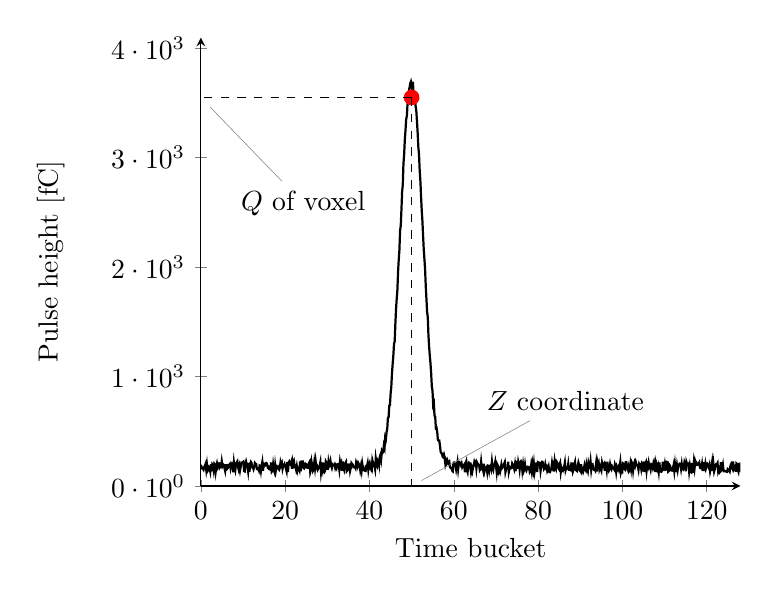
\begin{tikzpicture}
	\begin{axis}[
			% width=12cm, height=6cm,
			y tick label style={/pgf/number format/sci},
			ylabel style={yshift=10pt},
			xlabel={Time bucket}, ylabel={Pulse height [fC]},
			ymin=0, ymax=4096,
			domain=0:128, samples=800,
			axis lines=left
		]
		\addplot[thick] { (200 + 50 * (rand - 0.5) + 3500 * exp(-((x-50)^2)/15) }; % Random baseline + Gaussian peak
		\coordinate(peak) at (axis cs:50, 3500+50);
		\node[fill=red, circle, inner sep=2pt, thick] at (peak) {};
		\draw[dashed] (peak) -- (50, 0);
		\draw[dashed] (peak) -- (axis cs:0, 3500 +50);
		\node[pin={[pin distance=1cm]45:{$Z$ coordinate}}] at (axis cs:50, 0) {};
		\node[pin={[pin distance=1cm]-70:{$Q$ of voxel}}] at (axis cs:0, 3500 + 50) {};

	\end{axis}
\end{tikzpicture}

\section{ActRoot scheme}

\tikzsetnextfilename{actroot_scheme}
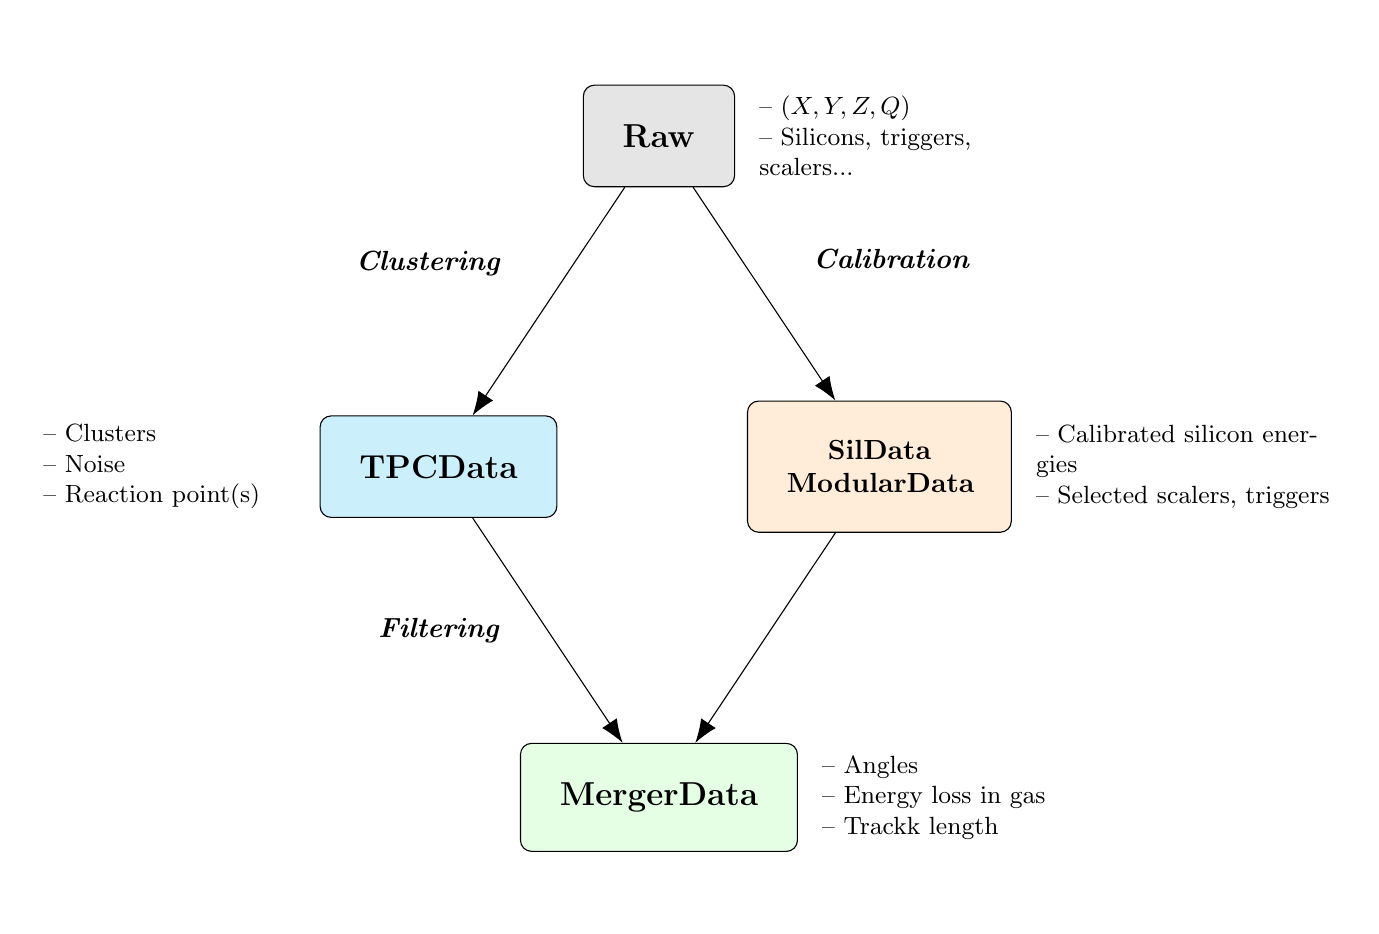
\begin{tikzpicture}[scale=0.7]
	\coordinate (a) at (0, 0);
	\coordinate (b) at (-4, -6);
	\coordinate (c) at (4, -6);
	\coordinate (d) at (0, -12);
	\node[draw, labelbox, fill=gray!20](raw) at (a) {\textbf{\large Raw}};
	\node[draw, textbox, right=0.1cm of raw] (textRaw) {
		\textendash\ $(X,Y,Z,Q)$\\
		\textendash\ Silicons, triggers, scalers...
	};
	\node[draw, labelbox, fill=cyan!20](tpc) at (b) {\textbf{\large TPCData}};
	\node[draw, textbox, left=-0.5cm of tpc](textTpc) {
		\textendash\ Clusters\\
		\textendash\ Noise\\
		\textendash\ Reaction point(s)};
  \node[draw, labelbox, fill=orange!15, text width=2.35cm](sil) at (c) {\textbf{SilData\\ModularData}};
	\node[textbox, right=0.1cm of sil](textSil){
		\textendash\ Calibrated silicon energies\\
		\textendash\ Selected scalers, triggers
	};
	\node[draw, labelbox, fill=green!10](merger) at (d) {\textbf{\large MergerData}};
	\node[textbox,right=0.1cm of merger](textMerger) {
		\textendash\ Angles\\
		\textendash\ Energy loss in gas\\
		\textendash\ Trackk length\\
	};
	%% Raw to TPC and Sil
	\draw[-{Latex[length=3mm]}] (raw) -- (tpc)
    node[midway, above left=0.2 and 0.5cm, actionbox] {Clustering};
	\draw[-{Latex[length=3mm]}] (raw) -- (sil)
    node[midway, above right=0.2 and 0.5cm, actionbox] {Calibration};
	%% Children to grandchild
	\draw[-{Latex[length=3mm]}] (tpc) -- (merger) 
    node[midway, above, left=0.0 and 0.5cm, actionbox] {Filtering};
	\draw[-{Latex[length=3mm]}] (sil) -- (merger);
\end{tikzpicture}
% \section{Filter}
% \subsection{BreakChi2}
%
% Initial approach:
%
% \tikzsetnextfilename{break_chi2_0}
% \begin{tikzpicture}
% 	\pic {actar};
%
% 	\pic (beam) {track={0/3/0/3/generic/}};
% 	\pic (light) {track={3/3/70/3.2/generic/}};
% 	\pic (heavy) {track={3/3/-10/3.1/generic/}};
%
% 	% define line coordinates
% 	\coordinate (up0) at (0, 3.2);
% 	\coordinate (up1) at (6, 3.2);
% 	\coordinate (low0) at (0, 2.8);
% 	\coordinate (low1) at (6, 2.8);
% 	\draw[very thick, line] (up0) -- (up1);
% 	\draw[very thick, line] (low0) -- (low1);
% \end{tikzpicture}
%
% After applying the breakchi2 operation:
%
% \tikzsetnextfilename{break_chi2_1}
% \begin{tikzpicture}
% 	\pic {actar};
%
% 	\pic (beam) {track={0/3/0/3/generic/}};
% 	\pic (light) {track={3/3/70/3.2/light/}};
% 	\pic (heavy) {track={3/3/-10/3.1/heavy/}};
%
% 	% define line coordinates
% 	\coordinate (up0) at (0, 3.2);
% 	\coordinate (up1) at (6, 3.2);
% 	\coordinate (low0) at (0, 2.8);
% 	\coordinate (low1) at (6, 2.8);
% 	\draw[very thick, line] (up0) -- (up1);
% 	\draw[very thick, line] (low0) -- (low1);
%
% 	\begin{scope}
% 		\clip (up0) -- (up1) -- (low1) -- (low0);  % Clip between the lines
% 		\pic (beam) {track={0/3/0/3/generic/}};
% 		\pic (light) {track={3/3/70/3.2/generic/}};
% 		\pic (heavy) {track={3/3/-10/3.1/generic/}};
% 	\end{scope}
% \end{tikzpicture}
%
% \subsection{Merge broken tracks}
%
% \tikzsetnextfilename{merge}
% \begin{tikzpicture}
% 	\pic {actar};
%
% 	\pic (beam) {track={0/3/0/3/generic/}};
% 	\pic (heavy) {track={3-0.1/3/-2/3.1/generic/}};
% 	\pic (light) {track={3/3/45/1.6/generic/true}};
% 	\pic (light) {track={4.25/4.25/47/2.4/generic/true}};
% \end{tikzpicture}
%
% \subsection{Pileup}
% \tikzsetnextfilename{pileup}
% \begin{tikzpicture}
%
% 	% define line coordinates
% 	\coordinate (up0) at (0, 4);
% 	\coordinate (up1) at (6, 4);
% 	\coordinate (low0) at (0, 2);
% 	\coordinate (low1) at (6, 2);
% 	\draw[very thick, line] (up0) -- (up1);
% 	\fill[orange!40] (up0) -- (up1) -- (6,6) -- (0,6) -- cycle;
% 	\draw[very thick, line] (low0) -- (low1);
% 	\fill[orange!40] (low0) -- (low1) -- (6,0) -- (0,0) -- cycle;
%
% 	\pic (beam) {track={0/3/0/6/generic/}};
% 	\pic (other) {track={0/5/0/6/gray/}};
% 	\pic (other) {track={0/1/0/6/gray/}};
%
% 	\pic {actar={Z}};
% \end{tikzpicture}
%
% \subsection{Fine analysis of tracks}
% It's going to be difficult to get the same images as Juan has


\end{document}
